\chapter{Relations, fonctions et produits cartésiens}

Dans ce chapitre, nous formaliserons les notions de relations, fonctions et de produits cartésiens quelconques. Ces notions nous sont essentiel afin de d'aborder l'axiome du choix et les différentes constructions des nombres usuels.

\section{Produit Cartésien de deux ensembles}

\begin{definition}[couple]
    Soient $a$ et $b$ deux ensembles, on définit le couple de $a$ et $b$ comme
    \[
    (a,b):= \{\{a\},\{a,b\}\}
    \]
\end{definition}

\begin{proposition}\label{couple: egalite}
    Le couple de $a$ et $b$ existe.
\end{proposition}

\begin{proof}
    Par \ref{ens: atoutseul}, $\{a\}$ existe. Dés lors, on applique l'axiome de la paire sur $a$ et $b$, ce qui nous garantit l'existence de $\{a,b\}$. Et enfin, on applique une nouvelle fois l'axiome de la paire sur $\{a\}$ et $\{a,b\}$ ce qui nous donne l'existence de $(a,b)$
\end{proof}

\begin{remarque}
    Remarquons que cette définition permet la non commutativité. C'est à dire que $(a,b)\neq (b, a)$. Cette manière de définir les couples est due à Kazimierz Kuratowski en 1921.
\end{remarque}

\begin{proposition}
    Soient $(a,b)$ et $(c,d)$ deux couples. On a
    \[
    (a,b)=(c,d) \Longleftrightarrow (a=c)\land(b=d)
    \]
\end{proposition}

\begin{proof}
    Si $a=c$ et $b=d$, alors on a trivialement que $(a,b)=(c,d)$. Supposons maintenant que $(a,b)=(c,d)$ et montrons que $a=c$ et que $b=d$. On a $\{a\}\in \{\{c\},\{c,d\}\}$ si $\{a\}=\{c\}$ alors $a=c$. Si $\{a\}=\{c,d\}$, nous devons distinguer deux cas. D'abord si $c=d$, alors $\{a\}=\{c\}$ et donc $a=c$. Maintenant si $c\neq d$, alors $\{c,d\}$ contient deux éléments distincts. Il ne peut donc pas être égal à $\{a\}$ qui ne contient qu'un élément. Cela contredit donc notre hypothèse. Ainsi, si $\{a\}=\{c,d\}$ alors $d=c$ et donc $a=c$ dans tous les cas. Il reste à montrer que $b=d$. on a $\{a,b\}\in \{\{c\},\{c,d\}\}$ donc $\{a,b\}=\{c\}$ ou $\{a,b\}=\{c,d\}$. Si $\{a,b\}=\{c,d\}$ alors $b=c$ ou $b=d$. Et si $c=b$ on a $b=c=a$ et donc $c=d$ sinon on aurait $\{a,b\} \neq \{c,d\}$ ainsi $b=d$. Et enfin, si $\{a,b\}=\{c\}$ alors $b=a=c$. Et $\{a\}=\{c,d\}$ donc $c=d$ et on trouve bien $b=d$.
\end{proof}

\begin{definition}[Produit cartésien]
Soient $A$ et $B$ deux ensembles, on définit le produit cartésien de $A$ et $B$ par
\[
A\times B := \{z\in \mathscr P( \mathscr P(A\cup B)) \mid \exists a\in A, \exists b\in B \: z=(a,b)\}
\]
\end{definition}
\begin{proposition}
    Le produit $A\times B$ existe 
\end{proposition}
\begin{proof}
    On sait par l'axiome de la réunion que $A\cup B$ existe et en appliquant deux fois l’axiome des parties, on déduit l'existence de $\mathscr P( \mathscr P(A\cup B))$. Cette argument combiné à l'existence des couples nous conduit à affirmer que la formule suivante est une formule du langage de ZF:
    \[
    \mathscr C(z,A,B)\equiv  \exists a\in A, \exists b\in B \: z=(a,b)
    \]
    Ainsi, par l'axiome de séparation $A\times B$ existe.
\end{proof}

\begin{remarque}
    Le lecteur pourrait se questionner quant à la raison d'une telle définition de $A\times B$. En effet, il peut sembler naturel de plutôt tenter de définir ce produit comme
    \[
    A\times B =\{(a,b)\in \mathscr P( \mathscr P(A\cup B)) \mid a\in A, b\in B \}.
    \]
    Cependant cette définition est trop informel pour pouvoir démontrer que cet ensemble existe à partir des axiomes. Il s'agit d'une définition naïve, on peut néanmoins, une fois après l'avoir définit formellement, utiliser cette approche comme une notation de l'ensemble $A\times B$. 
\end{remarque}

\section{Relations et fonctions}

\begin{definition}
    Une relation binaire (ou d'arité 2) entre deux ensembles $A$ et $B$ est un sous ensemble 
    \[
    R\subseteq A\times B.
    \]
\end{definition}

\begin{remarque}
    une relation binaire entre $A$ et $B$ peut être représenté par un ensemble de flèches reliant les éléments de \( A \) aux éléments de \( B \).
\end{remarque}

\begin{center} % Centrer tout le diagramme
	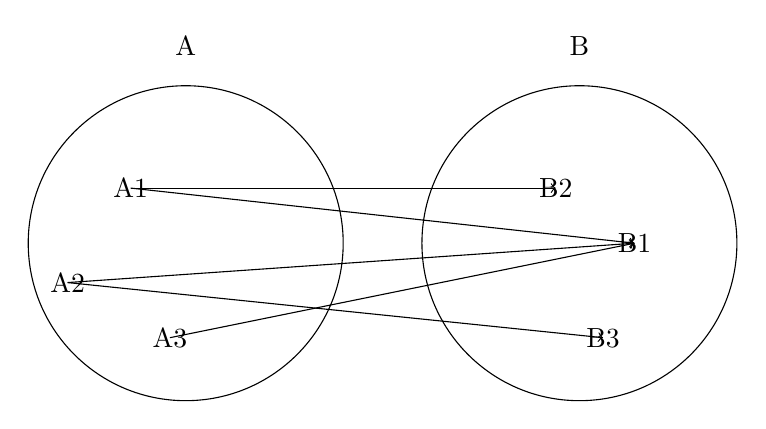
\begin{tikzpicture}

		% Ensemble A (cercle à gauche)
		\draw (0,0) circle (2cm);
		\node at (0, 2.5) {A};

		% Ensemble B (cercle à droite)
		\draw (5,0) circle (2cm);
		\node at (5, 2.5) {B};

		% Élément A1, A2, A3 dans A
		\node at (-0.7, 0.7) {A1};
		\node at (-1.5, -0.5) {A2};
		\node at (-0.2, -1.2) {A3};

		% Élément B1, B2, B3 dans B
		\node at (5.7, 0) {B1};
		\node at (4.7, 0.7) {B2};
		\node at (5.3, -1.2) {B3};

		% Flèches représentant la relation R (de A vers B)
		\draw[->] (-0.7, 0.7) -- (5.7, 0);  % A1 -> B1
		\draw[->] (-1.5, -0.5) -- (5.7, 0); % A2 -> B1
		\draw[->] (-0.2, -1.2) -- (5.7, 0); % A3 -> B1

		% Flèches supplémentaires pour illustrer d'autres relations
		\draw[->] (-0.7, 0.7) -- (4.7, 0.7);  % A1 -> B2
		\draw[->] (-1.5, -0.5) -- (5.3, -1.2); % A2 -> B3

	\end{tikzpicture}
\end{center}

\begin{notation}
    On écrit souvent $xRy$ au lieu de $(x,y)\in R$.
\end{notation}

\begin{definition}
    Soit $R\subseteq A\times B$ une relation binaire,
    \begin{itemize}
        \item Le \textbf{domaine} de $R$ est: $\dom (R) := \{a\in R \mid \exists b\in B, \: (a,b)\in R\}$
        \item L'\textbf{ image} de $R$ est: $\im (R):= \{b\in B \mid \exists a\in A, \: (a,b)\in R \}$
    \end{itemize}
\end{definition}

Par les même arguments que nous avons utilisés précédemment, il est facile de vérifier que ces ensembles existent.

\begin{definition}
	Soit \( R \) une relation binaire entre deux ensembles \( A \) et \( B \). La relation inverse \( R^{-1} \) est définie comme suit :

	\[
		R^{-1} \subseteq B \times A
	\]

	Plus précisément, si \( (a, b) \in R \), alors \( (b, a) \in R^{-1} \). En d'autres termes, la relation inverse consiste à inverser chaque paire de la relation \( R \).

	Formellement, si \( R \subseteq A \times B \), alors la relation inverse \( R^{-1} \subseteq B \times A \) est donnée par :

	\[
		R^{-1} = \{ (b, a) \mid (a, b) \in R \}
	\]
\end{definition}
On dit alors que $R^{-1}$ est l'inverse de $R$

\begin{definition}
    un graphe fonctionnelle $F$ de $A$ dans $B$ est une relation entre $A$ et $B$ vérifiant
    \[
    \forall x \in A, \forall y_1, y_2 \in B, [(x, y_1) \in F  \land  (x, y_2) \in F  \Rightarrow  y_2 = y_2]
    \]
\end{definition}

\begin{notation}
    Pour $(x,y)\in F$, on note généralement $F(x)=y$
\end{notation}

\begin{definition}
    Soit $F$ un graphe fonctionnel de $A$ dans $B$, on dit que 
    \begin{itemize}
        \item $F$ est une \textbf{application} si $\dom (F)= A$
        \item $F$ est \textbf{injectif} si $\forall x_1, x_2 \in \dom (F), [F(x_1) = F(x_2)  \Rightarrow  x_1 = x_1]$.
        \item $F$ est \textbf{surjectif} si $\forall y \in B, \exists x \in A, f(x) = y$ \textit{ i.e } $\im (F) = B$.
        \item $F$ est \textbf{bijectif} s'il est une application injective et surjective.
    \end{itemize}
\end{definition}
La notion d'injectivité est nous donne la propriété que $F$ est une correspondance "one to one". En terme de flèches, chaque éléments de $\dom(F)$ est relié à un seul élément de $Im(F)$.

\begin{proposition}
    Si $F$ est un graphe fonctionnel injectif alors $F^{-1}$ est un graphe fonctionnel.
\end{proposition}

\begin{proof}
Soit $F \subseteq A \times B$ injectif. Soient $y \in B$ et $x_1, x_2 \in A$ tels que 
$(y,x_1), (y,x_2) \in F^{-1}$. Par définition de $F^{-1}$, on a $(x_1,y), (x_2,y) \in F$. 
L'injectivité de $F$ implique $x_1 = x_2$. Donc $F^{-1}$ est fonctionnel.
\end{proof}

\begin{corollaire}
Si $F$ est un graphe fonctionnel bijectif alors $F^{-1}$ l'est aussi.
\end{corollaire}

\begin{proof}
Soit $F \subseteq A \times B$ bijectif, c'est-à-dire fonctionnel, injectif, avec 
$\mathrm{dom}(F) = A$ et $\mathrm{im}(F) = B$.

Par la proposition, $F^{-1}$ est fonctionnel. Montrons qu'il est aussi bijectif.

\textbf{Injectivité de $F^{-1}$.} Soient $y_1, y_2 \in B$ et $x \in A$ tels que 
$(y_1,x), (y_2,x) \in F^{-1}$. Alors $(x,y_1), (x,y_2) \in F$. Puisque $F$ est 
fonctionnel, $y_1 = y_2$.

\textbf{Domaine et image.} On a 
\begin{align*}
\mathrm{dom}(F^{-1}) &= \{y : \exists x, (x,y) \in F\} = \mathrm{im}(F) = B, \\
\mathrm{im}(F^{-1}) &= \{x : \exists y, (x,y) \in F\} = \mathrm{dom}(F) = A.
\end{align*}

Donc $F^{-1}$ est bijectif.
\end{proof}

\begin{definition}
    Soient $a$, $b$ et $c$ trois ensembles, on définit le triplet de $a$, $b$ et $c$ par
    \[
    (a,b,c):=((a,b),c)=\{\{\{\{a\},\{a,b\}\}\},\{\{\{a\},\{a,b\}\},c\}\}.
    \]
\end{definition}

\begin{remarque}
    Notons que, en général, $((a,b),c)\neq (a,(b,c))$ C'est pourquoi nous devons décider de la convention de $(a,b,c)$. Bien que $(a,b,c) := (a, (b,c))$ soit valable, nous suivrons la convention standard qui est celle ci-dessus.
\end{remarque}

\begin{proposition}
    Soient $a,b,c,a',b'$et $c'$ six ensembles. on a
    \[
    (a,b,c)=(a',b',c') \Longleftrightarrow (a=a')\land (b=b')\land (c=c')
    \]
\end{proposition}

\begin{proof}
    On a que $(a,b,c)=(a',b',c')$ est équivalent à $((a,b),c)=((a',b'),c')$. Par \ref{couple: egalite}, c'est équivalent à $((a,b)=(a',b'))\land (c=c')$. De même par \ref{couple: egalite}, c'est équivalent à $(a=a')\land (b=b')\land (c=c')$.
\end{proof}

\begin{definition}
    Une fonction $f$ de $A$ dans $B$ est un triplet $(F,A,B)$, où $A$ et $B$ sont des ensembles et $F$ est un graphe fonctionnel de $A$ dans $B$. On dit que $A$ est l'ensemble de départ de la fonction et que $B$ est l'ensemble d'arrivé.
\end{definition}

\begin{notation}
    On note une fonction de $f$ de $A$ dans $B$ par $f:A\to B$
\end{notation}

Cette définition nous permet d'établir que deux fonctions sont différentes si leur ensemble de départ ou d'arriver diffère et ce, même si leur graphe est identique.

\begin{definition}
    Soit $f=(F,A,B)$ une fonction.
    \begin{itemize}
        \item Le \textbf{domaine} de $f$ est: $\dom (f)= \dom (F)$.
        \item  L' \textbf{ image} de $f$ est: $\im (f) = \im (F)$.
        \item $f$ est \textbf{application} si $F$ l'est.
        \item $f$ est \textbf{injective} si $F$ l'est.
        \item $f$ est \textbf{surjective} si $F$ l'est.
        \item $f$ est une \textbf{bijection} si $F$ l'est.
    \end{itemize}
\end{definition}

\begin{remarque}
  D'un point de vue pratique, il est commode d'identifier une fonction à son graphe lorsqu'il n'y a pas de confusion possible. On pourrait définir $f(x)=y$ comme l'unique élément $y$ de $B$ tel que $(x,y)\in F$, cependant, il peut paraître un bonne chose de séparer les concepts d'"évaluation" et de fonction. Cette approche est également pratique pour certaine preuve, c'est donc l'approche que nous allons adopter.
\end{remarque}

\begin{definition}
    On définit
    $$B^A := \{F \in \mathcal{P}(A \times B) : F \text{ est un graphe fonctionnel de } A \text{ dans } B\}$$
\end{definition}

\begin{proposition}
    Soient $A$ et $B$ deux ensembles, $B^A$ existe.
\end{proposition}

\begin{proof}
On a
    \begin{enumerate}
\item $A \times B$ existe
\item $\mathcal{P}(A \times B)$ existe (axiome des parties)
\item La formule "$\forall x \in A \, \exists! y \in B \, (( x, y ) \in F)$" est une formule de $\mathcal{L}_{\text{ZF}}$
\item Par compréhension : $B^A = \{F \in \mathcal{P}(A \times B) \mid \forall x \in A ,\ \exists! y \in B ,\ ( x, y ) \in F\}$ existe.
\end{enumerate}
\end{proof}

\begin{remarque}
    Comme on identifie une fonction à son graphe, on peut considérer cet ensemble, comme l'ensemble des fonction de $A$ dans $B$.
\end{remarque}


\begin{definition}[Fonction d'évaluation]
Soient $A$ et $B$ deux ensembles. On définit la fonction d'évaluation :
$$\mathrm{ev}_{A,B} : A \times B^A \to B$$
par : pour tout $(x, F) \in A \times B^A$,
$$\mathrm{ev}_{A,B}(x, F) := \text{l'unique } y \in B \text{ tel que } (x,y) \in F.$$
\end{definition}

\begin{proposition}
La fonction $\mathrm{ev}_{A,B}$ est bien définie.
\end{proposition}

\begin{proof}
Soit $(x, F) \in A \times B^A$. Par définition de $B^A$, $F$ est un graphe fonctionnel 
de $A$ dans $B$, donc $\dom(F) = A$.

\textbf{Existence :} Puisque $x \in A = \dom(F)$, il existe $y \in B$ tel que $(x,y) \in F$.

\textbf{Unicité :} Si $(x,y_1) \in F$ et $(x,y_2) \in F$, alors par la propriété 
fonctionnelle de $F$, on a $y_1 = y_2$.

Donc $\mathrm{ev}_{A,B}(x,F)$ existe et est unique.
\end{proof}

\begin{definition}[Application d'une fonction]
Soit $f = (F, A, B)$ une fonction et $x \in A$. On définit :
$$f(x) := \mathrm{ev}_{A,B}(x, F).$$
\end{definition}

\begin{remarque}
La notation $f(x)$ est donc une \textbf{abréviation} pour $\mathrm{ev}_{A,B}(x, F)$, 
où $F$ est le graphe de $f$. Cela sépare formellement le concept de fonction (un triplet) 
du concept d'évaluation (une opération).
\end{remarque}

\begin{proposition}[Caractérisation de l'évaluation]\label{prop:eval-car}
Soit $f = (F, A, B)$ une fonction, $x \in A$, et $y \in B$. Alors :
$$f(x) = y \iff (x,y) \in F.$$
\end{proposition}

\begin{proof}
Découle immédiatement de la définition de $\mathrm{ev}_{A,B}$.
\end{proof}

\begin{proposition}[Extensionnalité]
Soient $f = (F, A, B)$ et $g = (G, A, B)$ deux fonctions de $A$ dans $B$. Alors :
$$f = g \iff \forall x \in A, f(x) = g(x).$$
\end{proposition}

\begin{proof}
($\Rightarrow$) Si $f = g$, alors $F = G$, donc pour tout $x \in A$, 
$f(x) = \mathrm{ev}_{A,B}(x, F) = \mathrm{ev}_{A,B}(x, G) = g(x)$.

($\Leftarrow$) Supposons $\forall x \in A, f(x) = g(x)$. Soit $(x,y) \in A \times B$ 
arbitraire. Par la proposition \ref{prop:eval-car} :
\begin{align*}
(x,y) \in F &\iff f(x) = y \\
&\iff g(x) = y \quad \text{(hypothèse)}\\
&\iff (x,y) \in G.
\end{align*}
Donc $F = G$, et par conséquent $f = g$.
\end{proof}

\section{Courbes de niveau}

\begin{definition}
	Soit \( F \) une fonction de \( A \to B \) et soit $b\in B$

	On appelle \textbf{courbes de niveau} de \( F \) l’ensemble :
	\[
		C_b (F)= \{ a \in A \mid F(a) = b \}
	\]
\end{definition}

Il est facile de vérifier que les courbes de niveaux existent

\begin{remarque}
	On a
	\begin{enumerate}
		\item  $F$ est \textbf{surjective} ssi $\forall b \in B $, \( C_b (F) \neq \emptyset \).
		\item \( F \) est \textbf{injective} ssi \( \forall b \in \im F \), \( C_b (F) \) est un singleton.
	\end{enumerate}
\end{remarque}

\begin{proposition}
	Soit $b,b'\in B$ et soient \( C_b (F) \) et \( C_{b'} (F) \) deux courbes de niveau de \( F \), alors soit elles sont \textbf{confondues}, soit elles sont \textbf{disjointes}.
\end{proposition}

\begin{proof}
	Soit \( x \in C_b(F) \cap C_{b'}(F) \), c'est-à-dire un élément appartenant à l'intersection des deux courbes de niveau. Par définition de ces ensembles, on a :
	\[
		F(x) = b \quad \text{et} \quad F(x) = b'.
	\]
	En conséquence, on obtient :
	\[
		b = b'.
	\]

	Cela signifie que si l'intersection \( C_b(F) \cap C_{b'}(F) \) est non vide, alors nécessairement \( b = b' \), ce qui implique que :
	\[
		C_b(F) = C_{b'}(F).
	\]

	Dans le cas contraire, si \( b \neq b' \), alors il n'existe aucun \( x \in A \) tel que \( F(x) = b \) et \( F(x) = b' \) simultanément, ce qui entraîne :
	\[
		C_b(F) \cap C_{b'}(F) = \emptyset.
	\]
\end{proof}

\section{Composition}
Après avoir, définit formellement les notions de fonction et de relation. Nous allons maintenant munir l'opération de composition à $B^A$.

\begin{definition}
    Soient $R\subseteq A\times B$ et $S\subseteq B\times C$ deux relations binaires. On définit la composition $S\circ R$ par
    \[
    S\circ R := \{(x,y)\in A\times C \mid \exists y\in B , \: [(x,y)\in R \land (y,z \in S)]\}
    \]
\end{definition}

\begin{proposition}
    Pour toutes relations $R \subseteq A \times B$ et $ S \subseteq B \times C$, l'ensemble $S \circ R$ existe.
\end{proposition}

\begin{proof}
Nous avons que
    $$\mathscr C(x, z, R, S, B) \equiv \exists y \in B, [(x,y) \in R \land  (y,z) \in S]$$
est une formule du premier ordre dans le langage de ZF, En effet, l'ensemble A × C existe puisque c'est un produit cartésien.
 Par l'axiome de séparation appliqué à $A \times C$ :
\[
S \circ R = \{(x,z) \in A \times C \mid \mathscr C(x, z, R, S, B)\}
\]
existe.
\end{proof}

\begin{proposition}
    Soient $R \subseteq A \times  B$ et $S \subseteq B \times C$ deux relations, alors $S \circ R \subseteq A \times C$ est une relation.
\end{proposition}

\begin{proof}
    Cela résulte directerment de la définition.
\end{proof}

\begin{proposition}
    
Soient $R \subseteq A \times B $et $S \subseteq B \times C$. Alors :

$$\dom (S \circ R) = \{x \in A \mid \exists y \in \im (R) \cap \dom (S), (x,y) \in R\}$$

En particulier, si $\dom (S) \supseteq \im (R)$, alors $\dom (S \circ R) = \dom (R)$.
\end{proposition}

\begin{proof}
    Soit $x\in A$, on a 
    \begin{align*}
        &x \in \dom (S \circ R)\\
\Leftrightarrow    &\exists z \in C, (x,z) \in S \circ R\\
\Leftrightarrow  &\exists z \in C, \exists y \in B, [(x,y) \in R \land (y,z) \in S]\\
\Leftrightarrow &\exists y \in B, [(x,y) \in R \land y \in \dom (S)]\\
\Leftrightarrow  &\exists y \in \im (R) \cap \dom (S), (x,y) \in R\\
    \end{align*}
\end{proof}

\begin{proposition}
    Soient $R \subseteq A \times B$ et $S \subseteq B \times C$. Alors :

$$\im (S \circ R) \subseteq \im (S)$$

Plus précisément : $\im (S \circ R) = S(\im (R))$ où $S(X) = \{z \in C\mid \exists y \in X, (y,z) \in S\}$.
\end{proposition}

\begin{proof}
    Soit $z \in \im (S \circ R)$. Alors :
\begin{align*}
&\exists x \in A, (x,z) \in S \circ R\\
\Leftrightarrow &\exists x \in A, \exists y \in B, [(x,y) \in R \land (y,z) \in S]\\
\Leftrightarrow &\exists y \in B, (y,z) \in S \\
\Leftrightarrow &z \in \im (S)
\end{align*}
\end{proof}

\begin{proposition}
    Soient $R\subseteq A\times B$, $S\subseteq B\times C$ et $T\subseteq C\times D$ trois relations. On a
    \[
    T\circ (S\circ R)= (T\circ S)\circ R.
    \]
    On dit que $\circ$ est associatif.
\end{proposition}

\begin{proof}
    Montrons l'égalité par double inclusion.

Soit $(x, w) \in A \times D$.

Supposons $(x, w) \in T \circ (S \circ R)$. Alors :
$$
\exists z \in C, [(x,z) \in S \circ R \land (z,w) \in T]
$$
Puisque $(x,z) \in S \circ R$ :
$$
\exists y \in B, [(x,y) \in R \land (y,z) \in S]
$$

Donc :
$$
\exists y \in B, \exists z \in C, [(x,y) \in R \land (y,z) \in S \land (z,w) \in T]
$$

Puisque $(y,z) \in S$ et $(z,w) \in T$: $(y,w) \in T \circ S$

Donc :
$$
\exists y \in B, [(x,y) \in R \land (y,w) \in T \circ S]
$$
C'est-à-dire $(x,w) \in (T \circ S) \circ R$. 

Supposons mainteant que $(x, w) \in (T \circ S) \circ R.$ Alors :
$$
\exists y \in B, [(x,y) \in R \land (y,w) \in T \circ S]
$$

Puisque $(y,w) \in T \circ S$ :
$$
\exists z \in C, [(y,z) \in S \land (z,w) \in T]
$$

Donc :
$$
\exists y \in B, \exists z \in C, [(x,y) \in R \land (y,z) \in S \land (z,w) \in T]
$$

Puisque $(x,y) \in R$ et $(y,z) \in S$ , on a
\[
(x,z) \in S \circ R
\]
Donc $\exists z \in C, [(x,z) \in S \circ R \land (z,w) \in T]$


C'est-à-dire $(x,w) \in T \circ (S \circ R)$. 
D'où $T \circ (S \circ R) = (T \circ S) \circ R.$ 

\end{proof}

On peut alors écrire $T \circ S \circ R$ sans ambiguïté.

\begin{definition}[Diagonale]
    Pour tout ensemble $A$, on définit la diagonale de A par :
    \[
    \Delta_A:=\{z\in A\times A\mid \exists x\in A, \: z=(x,x)\}
    \]
    Plus simplement on peut adopter la notation $\Delta_A= \{(x,x)\mid x\in A\}$
\end{definition}

\begin{proposition}
    Soit $A$ un ensemble, $\Delta_A$ existe.
\end{proposition}

\begin{proof}
    Cela vient du fait que la formule suivante est de ZF
    \[
    \mathscr C(z,A) \equiv \exists x\in A \: z=(x,x)
    \]
\end{proof}

\begin{proposition}
    Soit $R$ une relation entre $A$ et $B$, nous avons que 
    \begin{itemize}
        \item $\Delta_B\circ R=R$
        \item $R\circ \Delta_A=R$
    \end{itemize}
\end{proposition}

\begin{proof}
    Flemmememememem
\end{proof}

\begin{proposition}
    Soit $R\subseteq A\times B$ une relation, nous avons que
    \begin{itemize}
        \item $R\circ R^{-1}=\Delta_B$
        \item $R^{-1}\circ R=\Delta_A$
    \end{itemize}
\end{proposition}
\begin{proof}
    felmememeemlfemlflmeleflm
\end{proof}

\begin{proposition}
    Soient $F\subseteq A\times B$ et $G\subseteq B\times C$ deux graphes fonctionnels,
    $F\circ G$ est un graphe fonctionnel.
\end{proposition}

\begin{proof}
    flemme
\end{proof}
\begin{definition}
    Soient $f=(F,A,B)$ et $g=(G,B,C)$ deux fonctions, on définit la composition de $f$ et $g$ par $g\circ f:=(G\circ F,A,C)$.
\end{definition}
\begin{proposition}
    Soient $f=(F,A,B)$ et $g=(G,B,C)$ deux fonctions, $g\circ f$ est une fonction.

\end{proposition}

\begin{proposition}
    Soient $f = (F, A, B) : A \to B$ et $g = (G, B, C) : B \to C$ deux fonctions. Alors pour tout $x \in A$ :
$$(g \circ f)(x) = g(f(x)).$$
\end{proposition}


\begin{proof}
 
Notons $h = g \circ f = (G \circ F, A, C)$. Par définition de l'évaluation, on a 
$$h(x) = \mathrm{ev}_{A,C}(x, G \circ F),$$
c'est-à-dire l'unique $z \in C$ tel que $(x,z) \in G \circ F$.

Or, par définition de la composition de graphes,
$$(x,z) \in G \circ F \iff \exists y \in B, [(x,y) \in F \land (y,z) \in G].$$

Ainsi, $z$ est l'unique élément de $C$ pour lequel il existe $y \in B$ vérifiant $(x,y) \in F$ et $(y,z) \in G$.

Puisque $F$ est un graphe fonctionnel avec $\dom(F) = A$ et que $x \in A$, il existe un unique $y \in B$ tel que $(x,y) \in F$. Par définition de l'évaluation, cet élément $y$ n'est autre que $f(x)$.

Par conséquent, $z$ est l'unique élément de $C$ tel que $(f(x), z) \in G$. Par définition de l'évaluation, ceci signifie que
$$z = \mathrm{ev}_{B,C}(f(x), G) = g(f(x)).$$

On a donc bien $(g \circ f)(x) = g(f(x))$.
\end{proof}

\begin{definition}
    Pour tout ensemble A, on définit la \textbf{fonction identité} $\operatorname{id}_A : A \to A$ par :

\[\operatorname{id}_A := (\Delta_A, A, A)\]
\end{definition}

\begin{proposition}
    Pour tout ensemble $A$, $\operatorname{id}_A$ existe et est une fonction.
\end{proposition}

\begin{proof}
    Cela résulte du fait que $\Delta_A$ est un graphe fonctionnel.
\end{proof}

\begin{proposition}
    Pour toute fonction $f : A \to B$ :
    \begin{enumerate}
        \item $\operatorname{id}_B\circ f=f$
        \item $f\circ \operatorname{id}_A =f$
    \end{enumerate}
\end{proposition}

\begin{proposition}
    Soient $f:A\to B$ et $g:B\to C$ deux fonctions,
    \begin{enumerate}
        \item Si $f$ et $g$ sont injectives alors $g\circ f$ est injective.
        \item Si $f$ et $g$ sont surjectives alors $g\circ f$ est surjective.
        \item Si $f$ et $g$ sont bijectives alors $g\circ f$ est bijective.
    \end{enumerate}
\end{proposition}

Avec cette construction par l'évaluation on peut maintenant aborder la curryfication.




\section{Familles et produits cartésiens quelconques}

\begin{definition}
        Soit $I$ un ensemble, une famille indexée par $I$ est une couple $(E,A)$ où $E$ est un ensemble et $A$ une fonction de $I$ dans $E$.
    Pour tout $i \in I$, on note $A_i$ l'unique élément tel que $(i, A_i) \in A$, c'est-à-dire $A_i := A(i)$. On note souvent une telle famille $(A_i)_{i\in I}$.
\end{definition}

Par abus de langage, on identifie souvent la famille avec la fonction $A$ elle-même, mais formellement c'est le couple $(E, A)$.

\begin{definition}
        Soit $I$ un ensemble non vide et $(E, A)$ une famille
 indexée par $I$. On définit le produit cartésien de cette famille par :
        \[
        \prod_{i\in I}A_i:=\{f\in E^I \mid \forall i \in I, f(i)\in A_i\}
        \]
    \end{definition}

    \begin{proposition}
        Pour tout ensemble $I$ non vide et toute famille $(E, A)$ d'ensembles indexée par $I$, l'ensemble $\prod_{i\in I} A_i$ existe.
    \end{proposition}

    \begin{proof}
        Vu ce qui précède $E^I$ existe. De plus, Formule de compréhension : La formule

 $$\mathcal{C}(f, I, A) := \forall i \in I, (i, f(i)) \in f \land (i, A(i)) \in A \land f(i) \in A(i)$$
   est une formule du langage de ZF.

Application de l'axiome de séparation : Par l'axiome de compréhension, l'ensemble

 $$\prod_{i \in I} A_i = \{f \in E^I \mid \mathcal{C}(f, I, A)\}$$
   existe.
\end{proof}
\begin{remarque}
    On dira qu'une famille $(a_i)_{i\in I}$ est une \textbf{suite} si $I$ est un ensemble de la forme $\N^{\ge k}$
\end{remarque}
